\chapter{Proceso de desarrollo}
\label{capitulotres}
En este capitulo se explica, el proceso de desarrollo para la arquitectura de servicio web, se explicara como identificar el servicio, descripci'on de las etapas y procesos.

Para usar los servicios web, debemos conocer donde se ubica, los detalles de la interfaz todo esto se detalla en la descripci'on de servicio.
\section{Descripci'on del Servicio}
El servicio web, se tiene que conocer la ubicac'ion, los detalles de la interfaz para esto se realiza algunas preguntas seg'un \cite{Somerville2011}.
Se define en las partes de:
\begin{enumerate}
\item [Que:] Se realiza un documento llamado interfaz es donde, se define las operaciones que soporta el servicio y define el formato de los mensajes que se env'ian y reciben por parte del servicio.
\item [Como:] Se realiza un documento llamado enlace, mapea la interfaz abstracta a un conjunto concreto de protocolos, especifica los detalles t'ecnicos de c'omo comunicarse con un servicio.
\item [Donde:] Se realiza un documento, en donde se describe la ubicaci'on de la implementaci'on del servicio web en su punto final.
\end{enumerate}

El servicio web debe calcular que hace realmente que significa cada campo en los mensajes de entrada y salida.

Para la comunicaci'on de servicio web se utiliza los siguientes protocolos.

\section{Protocolos }
Los servicios web, nos apoyan a trabajar en la comunicaci'on, para proporcionar servicios integrales de comunicaci'on de red. El c'ual, cubren todos los aspectos del SOA, desde los mecanismos b'asicos, para el intercambio de informac'ion con los protocolos est'andares y no est'andar de informaci'on de lenguaje, los cuales son: SOAP, WSDL, WS-BPEL, REST.
Para este proyecto se ha utilizado el protocolo no estandar el servicio REST.
\section{Representaci'on est'andar de transferencia -REST} 
El REST es un protocolo, basado en est'andares, mediante restricci�n de establecer la interfaz a un conjunto conocido de operaciones est�ndar (por ejemplo GET, PUT,...). Por tanto, este estilo se centra m�s en interactuar con recursos con estado, que con mensajes y operaciones.
\begin{figure}[H]
\centering
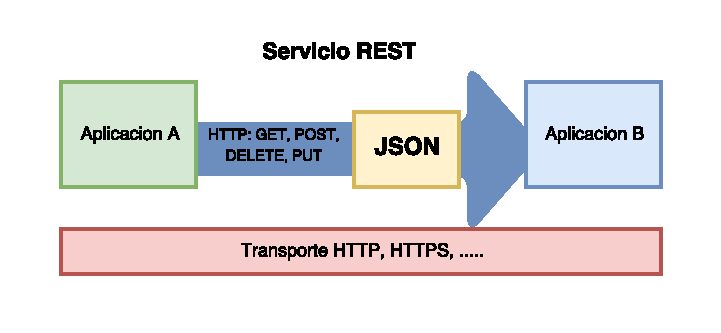
\includegraphics[width=0.6\textwidth]{servicioREST.pdf}
\captionsetup{justification=centering,margin=2cm}
\caption{Representaci'on del servicio REST, adoptado para la realizac'ion del proyecto. Servicio REST\cite{Blancarte2017}}
\end{figure}

Despues de la descripci'on de datos, se pasa a conocer la ingenier'ia de servicio, que nos ayudara en  el proceso de desarrollo de servicio para aplicaci'ones orientadas a servicios.

\section{Ingenier'ia de servicio}

La ingenier'ia de servicio es el proceso, de desarrollo de servicios para reutulizaci'on en aplicaciones orientadas a servicios, es aqui donde se debe garantizar que el servicio represente una abstracci'on de reutilizaci'on, que podr'ia ser 'util para que el servicio sea robusto y fiable. Existe las siguiente etapa en la siguiente \ref{DiagramaIngenieria}: 

\begin{figure}[H]
\centering
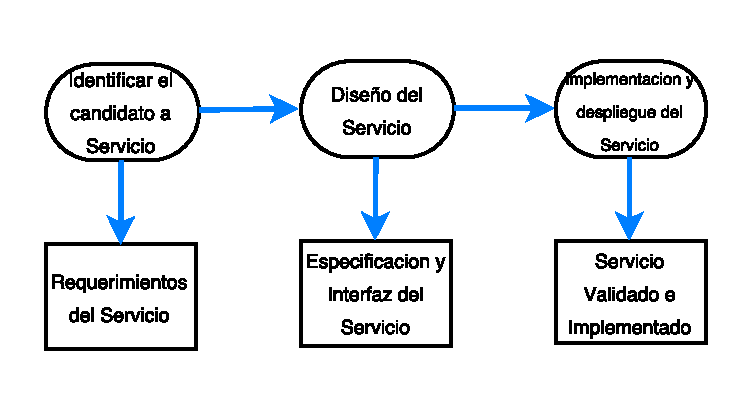
\includegraphics[width=0.6\textwidth]{procesoServicio.pdf}
\captionsetup{justification=centering,margin=2cm}
\caption{El proceso de ingenier'ia de servicio, adoptado para la realizac'ion del proyecto. El proceso de ingenier'ia de servicio\cite{Sommerville2012}}
\label{DiagramaIngenieria}
\end{figure}

Cada proceso de desarrollo de la ingenier'ia, se define en:
\begin{enumerate}
\item Identificador de candidatos a servicio, donde se identifican los posibles servicios que se pueden implementar y se define, los requerimiento del servicio.
\item Dise'no del servicio, donde se dise'na la interfaz l'ogica y de servicio.
\item Implementaci'on y se depliegue del servicio, donde el servicio se implementa,  se prueba y se pone a disposici'on del usuario.
\end{enumerate}

El punto de partida, para el proceso del servicio, es un servicio existente, o un componente que se convertir'a en servicio.

\subsection{Identificaci'on de candidatos a servicio}
Para identificar, los candidatos a servicio implica comprender y analizar los procesos empresariales de la organizaci'on para decidir c'ual servicio se podr'ian reutilizar para implementar para soportar dicho proceso. Se tiene 3 tipos de servicios son: utilitarios, empresariales y coordinaci'on o proceso.

Para el presente proyecto, se ha elegido un servicio empresarial, que se explica a continuaci'on.

\begin{itemize}
\item Servicio empresarial, se trata de servicios asociados, con una funci'on empresarial especifica. Un ejemplo de una funci'on empresarial es una universidad ser'ia la inscripci'on de estudiantes para un curso. 
\end{itemize}

Los servicios pueden ser orientados a entidades, que son como objetos y orientados a  tareas, que son aquellas asociadas con alguna actividad. Para seleccionar el servicio, se plantean los siguientes preguntas. 
\begin{enumerate}
\item El servicio de entidades esta asociado, con una solo entidad l'ogica que se usa en diferentes procesos empresariales?
\item Que operaciones que deban soportarse se realizan usualmente sobre dicha entidad?
\item Se trata de tareas que realizan diferentes personas en la organizaci'on?
\item El servicio es independiente?
\item El servicio tiene estado?
\item El servicio pueden usarlo, clientes fuera de la organizaci'on?
\item Diferentes usuarios, tienen distintos requerimientos?
\end{enumerate}

El resultado  del proceso de selecci'on, son un conjunto de servicios identificados y la lista de requerimientos funcionales del servicio, es lo que debe definir que debe hacer el servicio. Los requerimientos no funcionales deben definir los requerimientos de seguridad, rendimiento y disponibilidad del servicio.

\subsection{Dise'no de interfaces del servicio}
Una vez concluido la selecci'on del servicio, despu'es se realizara las operaciones asociadas con el servicio y sus p'arametros, el dise'no de operaciones y los mensajes de servicio. El dise'no se representa en 3 etapas: 
\begin{enumerate}
\item \textbf{Dise'no de interfaz logica,} se identifica las operaciones asociadas con el servicio, sus entradas y salidas, as'i como las excepciones asociadas con dichas operaciones. Empieza con los requerimientos del servicio, define los nombres y parametros de operaci'on. Se debe definir las excepciones que s'urgen cuando se ubica una operaci'on de servicio.
\item \textbf{Dise'no de mensajes,} donde se dese'na la estructura de los mensajes que env'ia y recibe el servicio. Se define los mensajes de entrada y salida, se debe manejar los mensajes como objetos, tiene la estructura en operaci'on, entradas, salidas y excepciones.
\item \textbf{Dise'no l'ogico,} comienza con una instrucci'on de interfaz abstracta.
\end{enumerate}
Una vez concluido, con el dise'no, se realiza la implementaci'on.

\subsection{Implementaci'on y despliegue de servicio}
 La implementaci'on implica la programaci'on de dicho servicio, en alg'un lenguaje que te permita realizar servicio. Despu'es se debe probar, con la participaci'on de las entradas del servicio y as'i generando excepciones, durante la prueba.  

La etapa del desarrollo de software para construir el servicio web.

\section{Desarrollo de software con servicios}
 
El desarrollo de software es combinar y configurar servicios, para crear nuevos servicios compuestos. Los nuevos servicios, son nuevas composiciones de servicios que pueden usarse  para dar un proceso integrado que ofrezca funcionalidad mas extensa. Este proceso es como una secuencia de pasos denominada como flujo de trabajo.
\subsection{Flujo de trabajo}
El flujo de trabajo es  es un conjunto de actividades orientadas en que cada actividad realiza parte del trabajo. Es el c'ual establece los pasos necesarios para alcanzar una meta particular.
\subsection{Acci'on de compensaci'on}
La acci'on de compensaci'on se utilizan para deshacer acciones que ya se completaron, el c'ual deben cambiar el resultado de posteriores actividades del flujo de trabajo.

%(8-10pp)